\chapter*{}
%\thispagestyle{empty}
%\cleardoublepage

%\thispagestyle{empty}

\begin{titlepage}
 
 
\setlength{\centeroffset}{-0.5\oddsidemargin}
\addtolength{\centeroffset}{0.5\evensidemargin}
\thispagestyle{empty}

\noindent\hspace*{\centeroffset}\begin{minipage}{\textwidth}

\centering
%
\includegraphics[width=0.9\textwidth]{imagenes/logo_ugr.jpg}\\[1.4cm]

%\textsc{ \Large PROYECTO FIN DE CARRERA\\[0.2cm]}
%\textsc{ INGENIERÍA EN INFORMÁTICA}\\[1cm]
% Upper part of the page
% 

 \vspace{3.3cm}

%si el proyecto tiene logo poner aquí
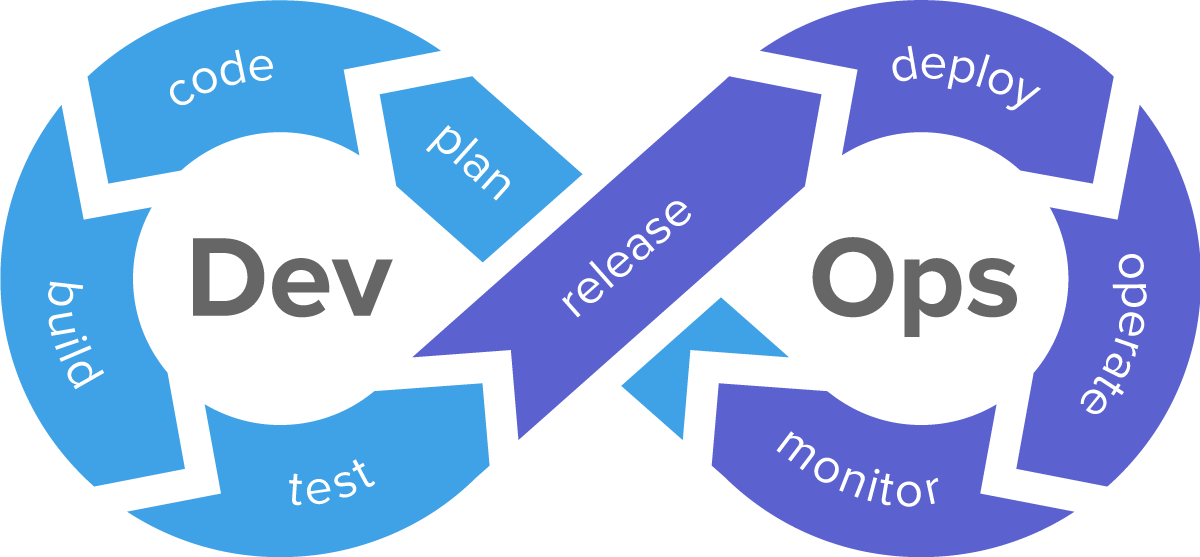
\includegraphics[width=0.9\textwidth]{imagenes/logo4.png}\\[1.4cm]
 \vspace{0.5cm}

% Title

{\Huge\bfseries Despliegue automático de infraestructura + CI/CD\\
}
\noindent\rule[-1ex]{\textwidth}{3pt}\\[3.5ex]
{\large\bfseries Implementación de técnicas DevOps \\[4cm]}
\end{minipage}

\vspace{2.5cm}
\noindent\hspace*{\centeroffset}\begin{minipage}{\textwidth}
\centering

\textbf{Autor}\\ {Víctor Moreno Jiménez}\\[2.5ex]
\textbf{Directores}\\
Juan Julián Melero Guervós \\[2cm]
%
\includegraphics[width=0.15\textwidth]{imagenes/tstc.png}\\[0.1cm]
%\textsc{Departamento de Teoría de la Señal, Telemática y Comunicaciones}\\
%\textsc{---}\\
%Granada, mes de 201
\end{minipage}
%\addtolength{\textwidth}{\centeroffset}
\vspace{\stretch{2}}

 
\end{titlepage}





\cleardoublepage
\thispagestyle{empty}

\begin{center}
{\large\bfseries  Despliegue automático de infraestructura + CI/CD: Implementación de técnicas DevOps}\\
\end{center}
\begin{center}
Víctor Moreno Jiménez\\
\end{center}

%\vspace{0.7cm}
\noindent{\textbf{Palabras clave}: DevOps, IaC (Infraestructure as Code), CI (Continous Integration), CD (Continous Delivery)}\\

\vspace{0.7cm}
\noindent{\textbf{Resumen}}\\

El objectivo de este TFG es conseguir un ciclo rápido y replicable de la infraestructura de una pequeña empresa así como conseguir crear un ciclo de creación y despliegue de aplicaciones. 

\bigskip 
En concreto se va a automatizar todo el proceso de despliegue de infraestructura (IaC) y se van a aplicar los principios de integración contínua y entrega contínua propios de la filosofía DevOps en todo el ciclo de desarrollo de los productos de la empresa. La finalidad de esto es poder disponer de una infraestructura segura y facilmente recreable en caso de catástrofe o ampliación del cluster. Desde el punto de vista de los desarrolladores de la empresa, podrán tener a su disposición y bajo demanda, un entorno de desarrollo mediante ficheros de configuración sin depender directamente del departamento de sistemas. \bigskip

Este proyecto supone una mejora técnica en la creación y despliegue de infraestructura de la empresa.

\cleardoublepage


\thispagestyle{empty}


\begin{center}
{\large\bfseries Automatic deployment of infrastructure + CI / CD: Implementation of DevOps techniques}\\
\end{center}
\begin{center}
Víctor Moreno Jiménez\\
\end{center}

%\vspace{0.7cm}
\noindent{\textbf{Keywords}: DevOps, IaC (Infraestructure as Code), CI (Continous Integration), CD (Continous Delivery)}\\

\vspace{0.7cm}
\noindent{\textbf{Abstract}}\\

The main goal of this project is to achieve a fast and replicable cycle of infraestructure in a small company, as well as to create a cycle of creation and deployment of applications. \bigskip

The entire company infraestructure will be automated using some orchestration tools via configuration files (Infrastructure as Code). Continuous integration and continuous deployment will be used to create development pipelines. \bigskip

The purpose of this is to be able to have a secure and easily deployable infrastructure. From the point of view of the company's developers, they will have the ability to create development infrastructures on demand without depending directly on the systems department.

This project is a technical improvement in creation and deployment of the infraestructure of the company.
\bigskip


\chapter*{}
\thispagestyle{empty}

\noindent\rule[-1ex]{\textwidth}{2pt}\\[4.5ex]

Yo, \textbf{Victor Moreno Jiménez}, alumno de la titulación Ingeniería Informática de la \textbf{Escuela Técnica Superior
de Ingenierías Informática y de Telecomunicación de la Universidad de Granada}, con DNI 47252942V, autorizo la
ubicación de la siguiente copia de mi Trabajo Fin de Grado en la biblioteca del centro para que pueda ser
consultada por las personas que lo deseen.

\vspace{6cm}

\noindent Fdo: Víctor Moreno Jiménez

\vspace{2cm}

\begin{flushright}
Granada a 31 de Julio de 2020.
\end{flushright}


\chapter*{}
\thispagestyle{empty}

\noindent\rule[-1ex]{\textwidth}{2pt}\\[4.5ex]

D. \textbf{Juan Julián Merelo Guervós}, Profesor del Área de XXXX del Departamento YYYY de la Universidad de Granada.


\vspace{0.5cm}

\textbf{Informan:}

\vspace{0.5cm}

Que el presente trabajo, titulado \textit{\textbf{Automatic deployment of infrastructure + CI / CD: Implementation of DevOps}},
ha sido realizado bajo su supervisión por \textbf{Víctor Moreno Jiménez}, y autorizamos la defensa de dicho trabajo ante el tribunal
que corresponda.

\vspace{0.5cm}

Y para que conste, expiden y firman el presente informe en Granada a 25 de Agosto de 2020.

\vspace{1cm}

\textbf{Los directores:}

\vspace{5cm}
\noindent Fdo: Juan Julián Merelo Guervós



\chapter*{Agradecimientos}
\thispagestyle{empty}

       \vspace{1cm}


Para toda la gente maravillosa que me he cruzado en estos 4 años de carrera. No habría sido lo mismo sin vosotros... Gracias

